\documentclass[
    a4paper
]{scrreprt}
\usepackage[ngerman]{babel}
\usepackage[utf8]{inputenc}
\usepackage{textcomp, expdlist, array, colortbl, xcolor}
\usepackage[pdftex]{graphicx}
\usepackage[TS1, T1]{fontenc}
\usepackage{palatino} % Schriftart
\usepackage{parskip} %Erste Zeile eines Paragrafen nicht einrücken

\usepackage{listings}
\usepackage{color}
\usepackage{xcolor}

\colorlet{punct}{red!60!black}
\definecolor{background}{HTML}{EEEEEE}
\definecolor{delim}{RGB}{20,105,176}
\colorlet{numb}{magenta!60!black}
\definecolor{mygreen}{rgb}{0,0.6,0}

\lstdefinelanguage{json}{
	basicstyle=\normalfont\ttfamily,
	stepnumber=1,
	numbersep=8pt,
	showstringspaces=false,
	breaklines=true,
	backgroundcolor=\color{background},
	morestring=[s][\color{red}]{"}{"},
	morekeywords={set, hash, key, list},
	morecomment=[l]{//},
	literate=
	*{0}{{{\color{numb}0}}}{1}
	{1}{{{\color{numb}1}}}{1}
	{2}{{{\color{numb}2}}}{1}
	{3}{{{\color{numb}3}}}{1}
	{4}{{{\color{numb}4}}}{1}
	{5}{{{\color{numb}5}}}{1}
	{6}{{{\color{numb}6}}}{1}
	{7}{{{\color{numb}7}}}{1}
	{8}{{{\color{numb}8}}}{1}
	{9}{{{\color{numb}9}}}{1}
	{:}{{{\color{punct}{:}}}}{1}
	{,}{{{\color{punct}{,}}}}{1}
	{\{}{{{\color{delim}{\{}}}}{1}
	{\}}{{{\color{delim}{\}}}}}{1}
	{[}{{{\color{delim}{[}}}}{1}
	{]}{{{\color{delim}{]}}}}{1}
	{1aba56d8c5}{{{\color{numb}1aba56d8c5}}}{10}
}

\lstset{
	language={json},
	commentstyle=\color{mygreen}
}


\begin{document}
    \sffamily % Whole document sans-serif


    % Titelseite
    \begin{titlepage}
        \centering
        
\includegraphics[width=0.8\textwidth]{./images/logo_hska.png}\par\vspace{1cm}
        \vspace{1cm}

        {\scshape\Large Verteile Systeme 2 -- Labor\par}
        \vspace{1.5cm}

        {\huge\textbf{Twitter-Klon}\par}
        \vspace{2cm}

        {\Large\itshape Timo Blust, 48594\par}
        {\Large\itshape Gennadi Eirich, 50629\par}
        {\Large\itshape Tim Essig, 49683\par}
        {\Large\itshape Maike Rees, 47307\par}

        \vfill

        % Bottom of the page
        {\large \today\par}
    \end{titlepage}


    % Inhaltsverzeichnis
    \tableofcontents


    % Aufgabe 1
    \chapter{Konzeption und Gestaltung}
    \section{Use Case Diagramm}
    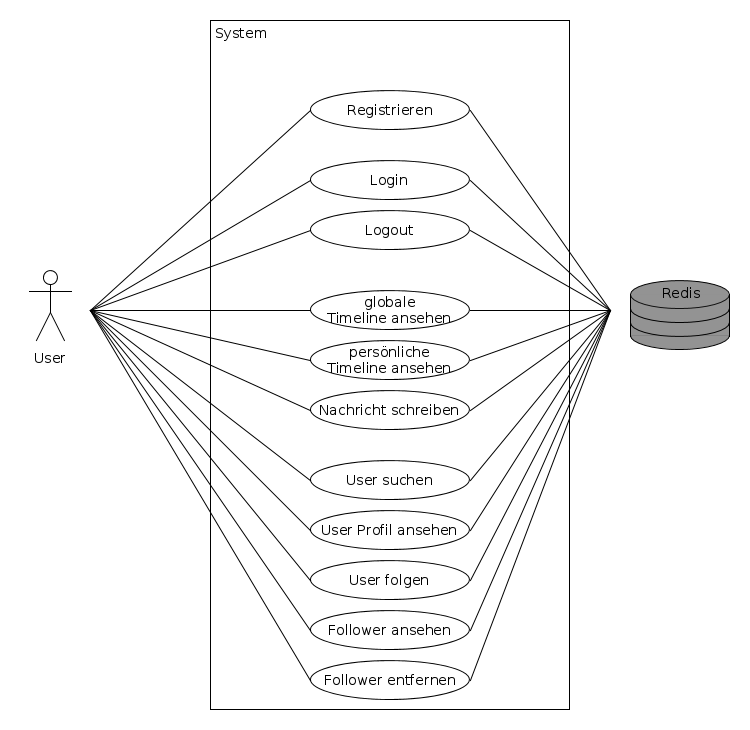
\includegraphics[width=\textwidth]{./images/useCaseDiagramm.png}

    \section{Entwurf der Seitennavigation}
	     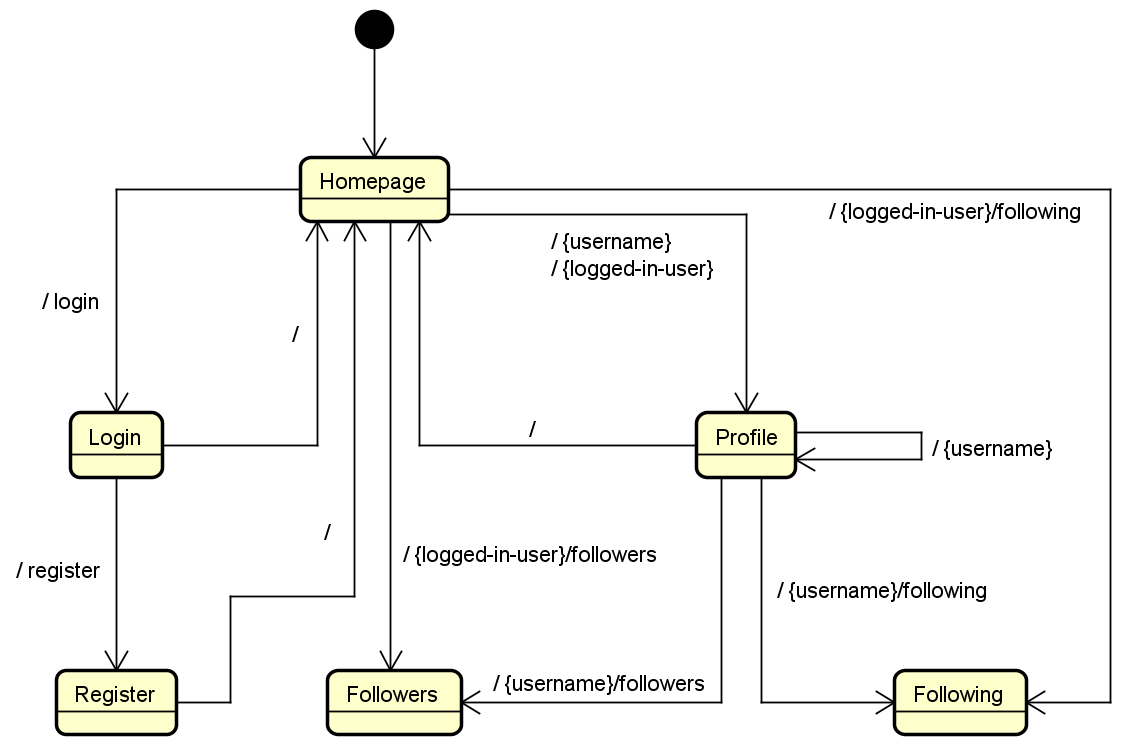
\includegraphics[width=\textwidth]{./images/state-machine.png}

    \section{Mockup}
		\includegraphics[width=\textwidth]{./images/1_login.png}
		Login\par\vspace{.6cm}
		\includegraphics[width=\textwidth]{./images/1_registration.png}
		Registration\par\vspace{.6cm}
		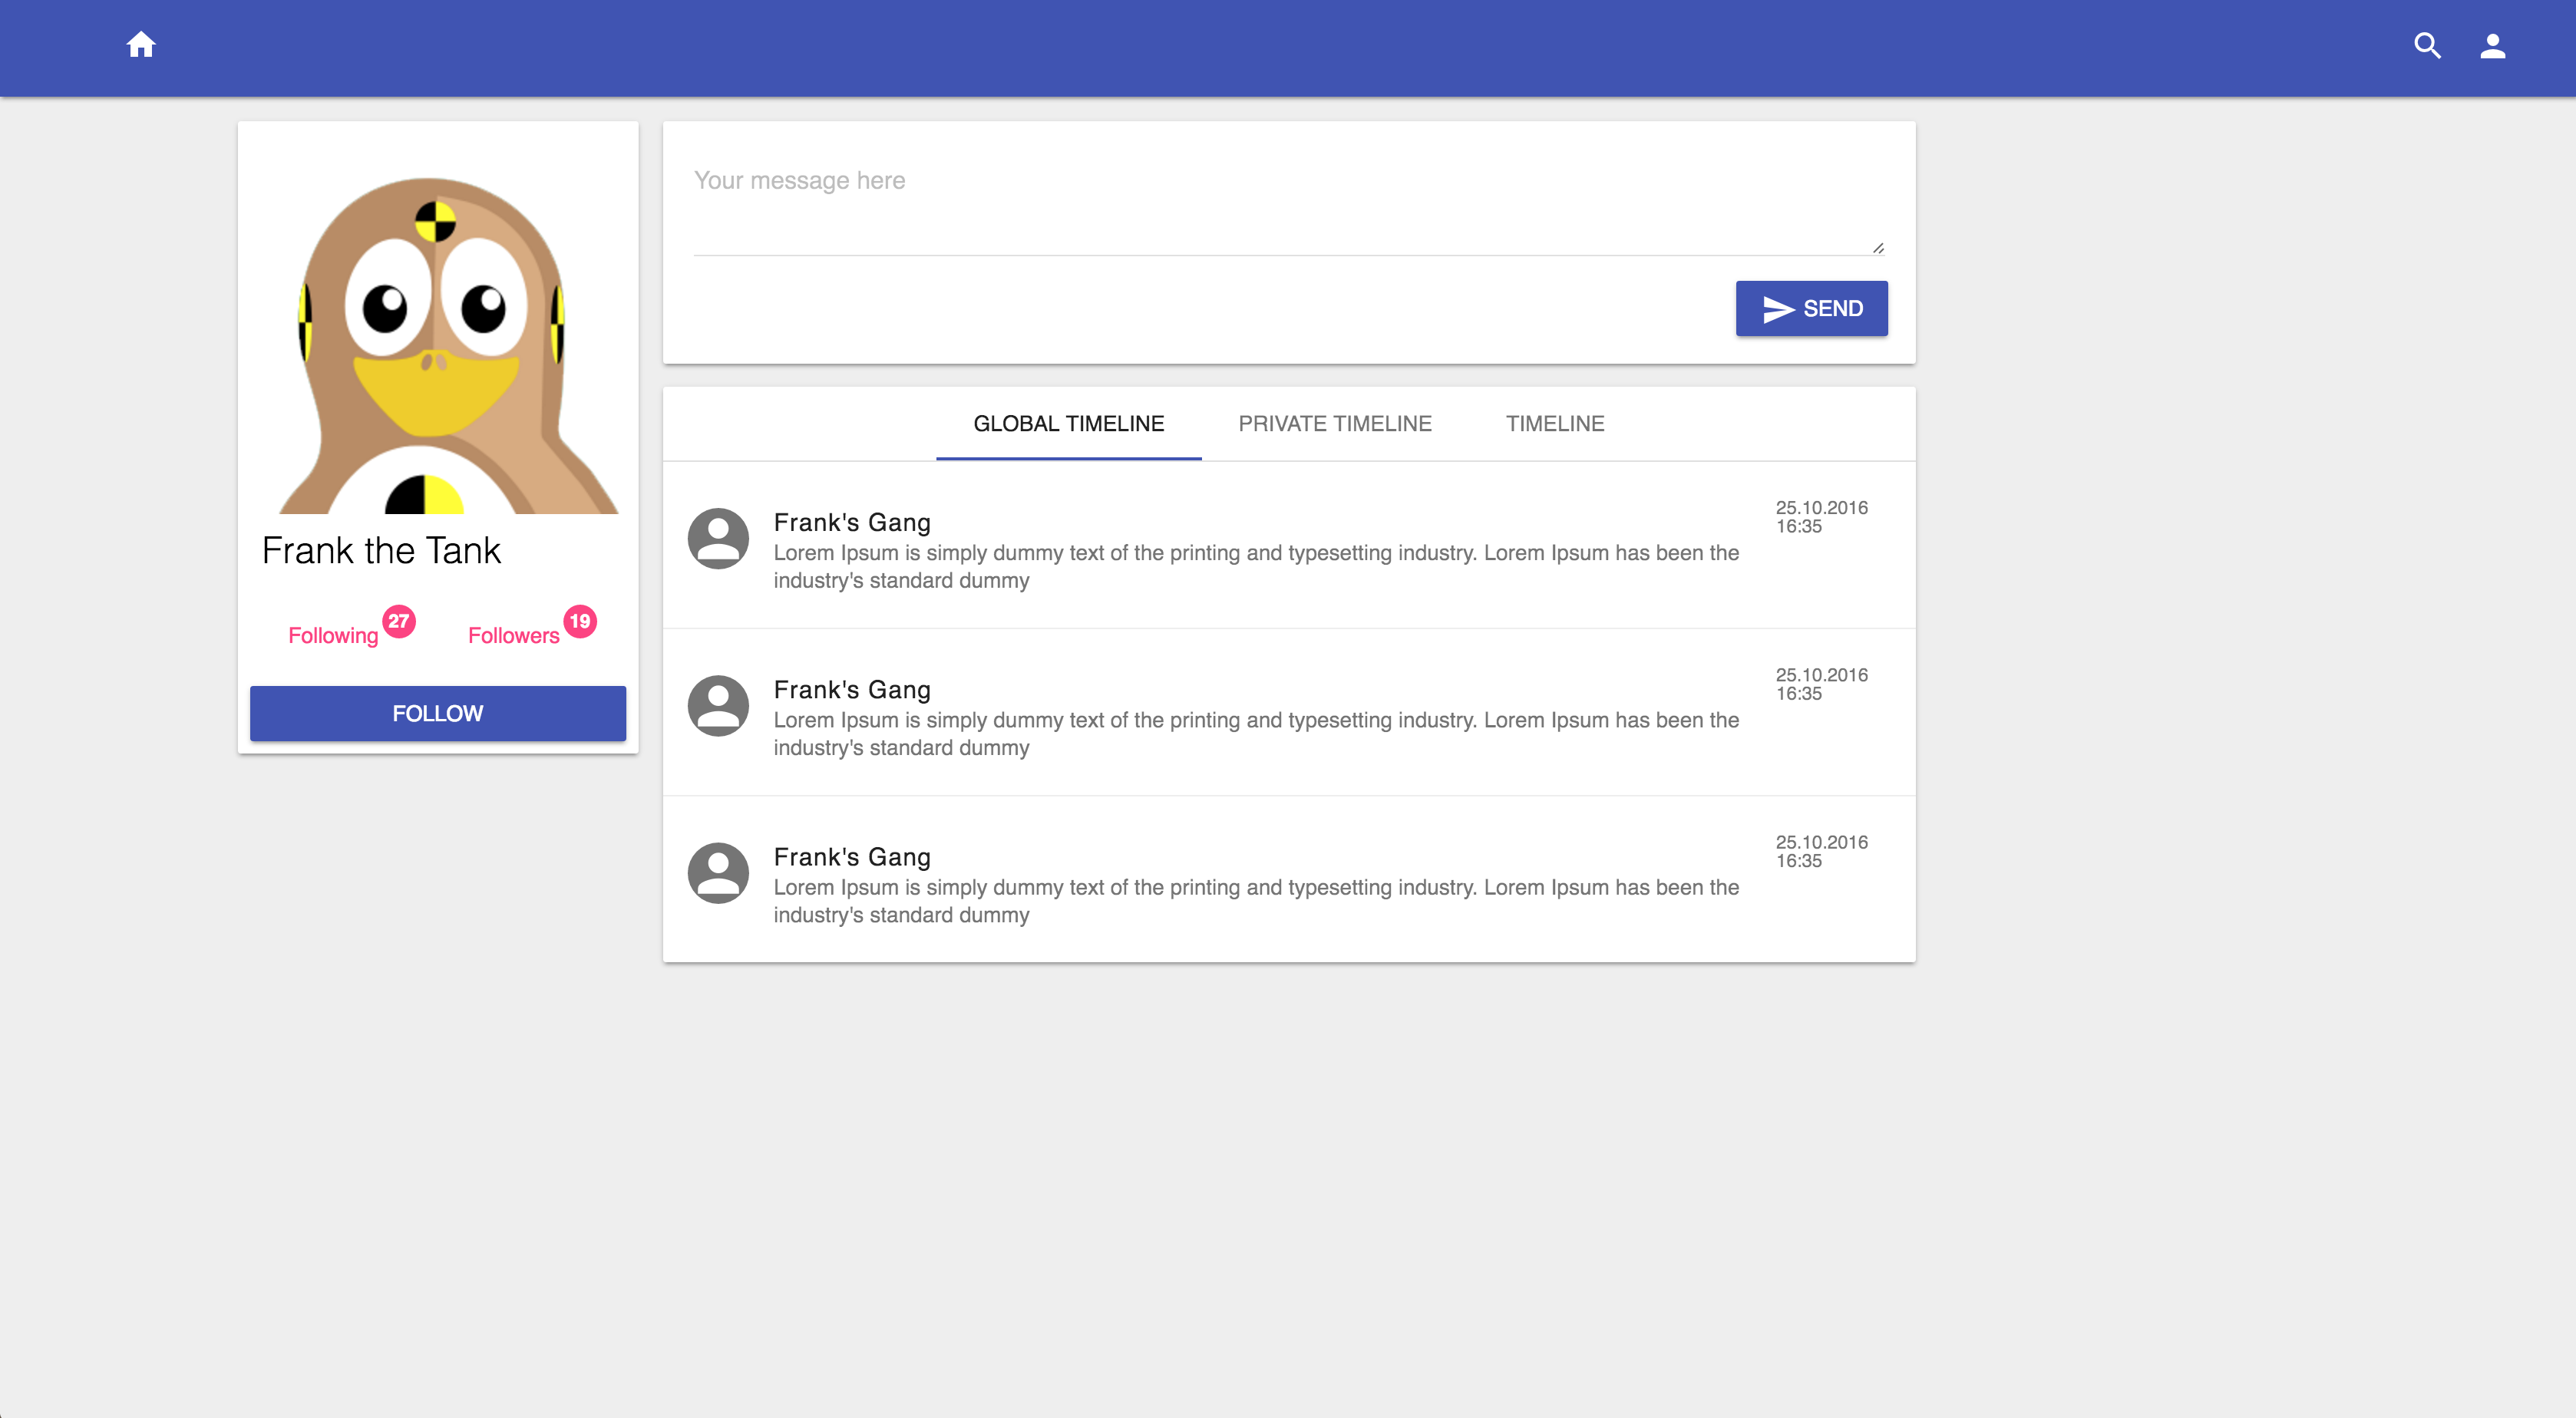
\includegraphics[width=\textwidth]{./images/1_home.png}
		Home\par\vspace{.6cm}
		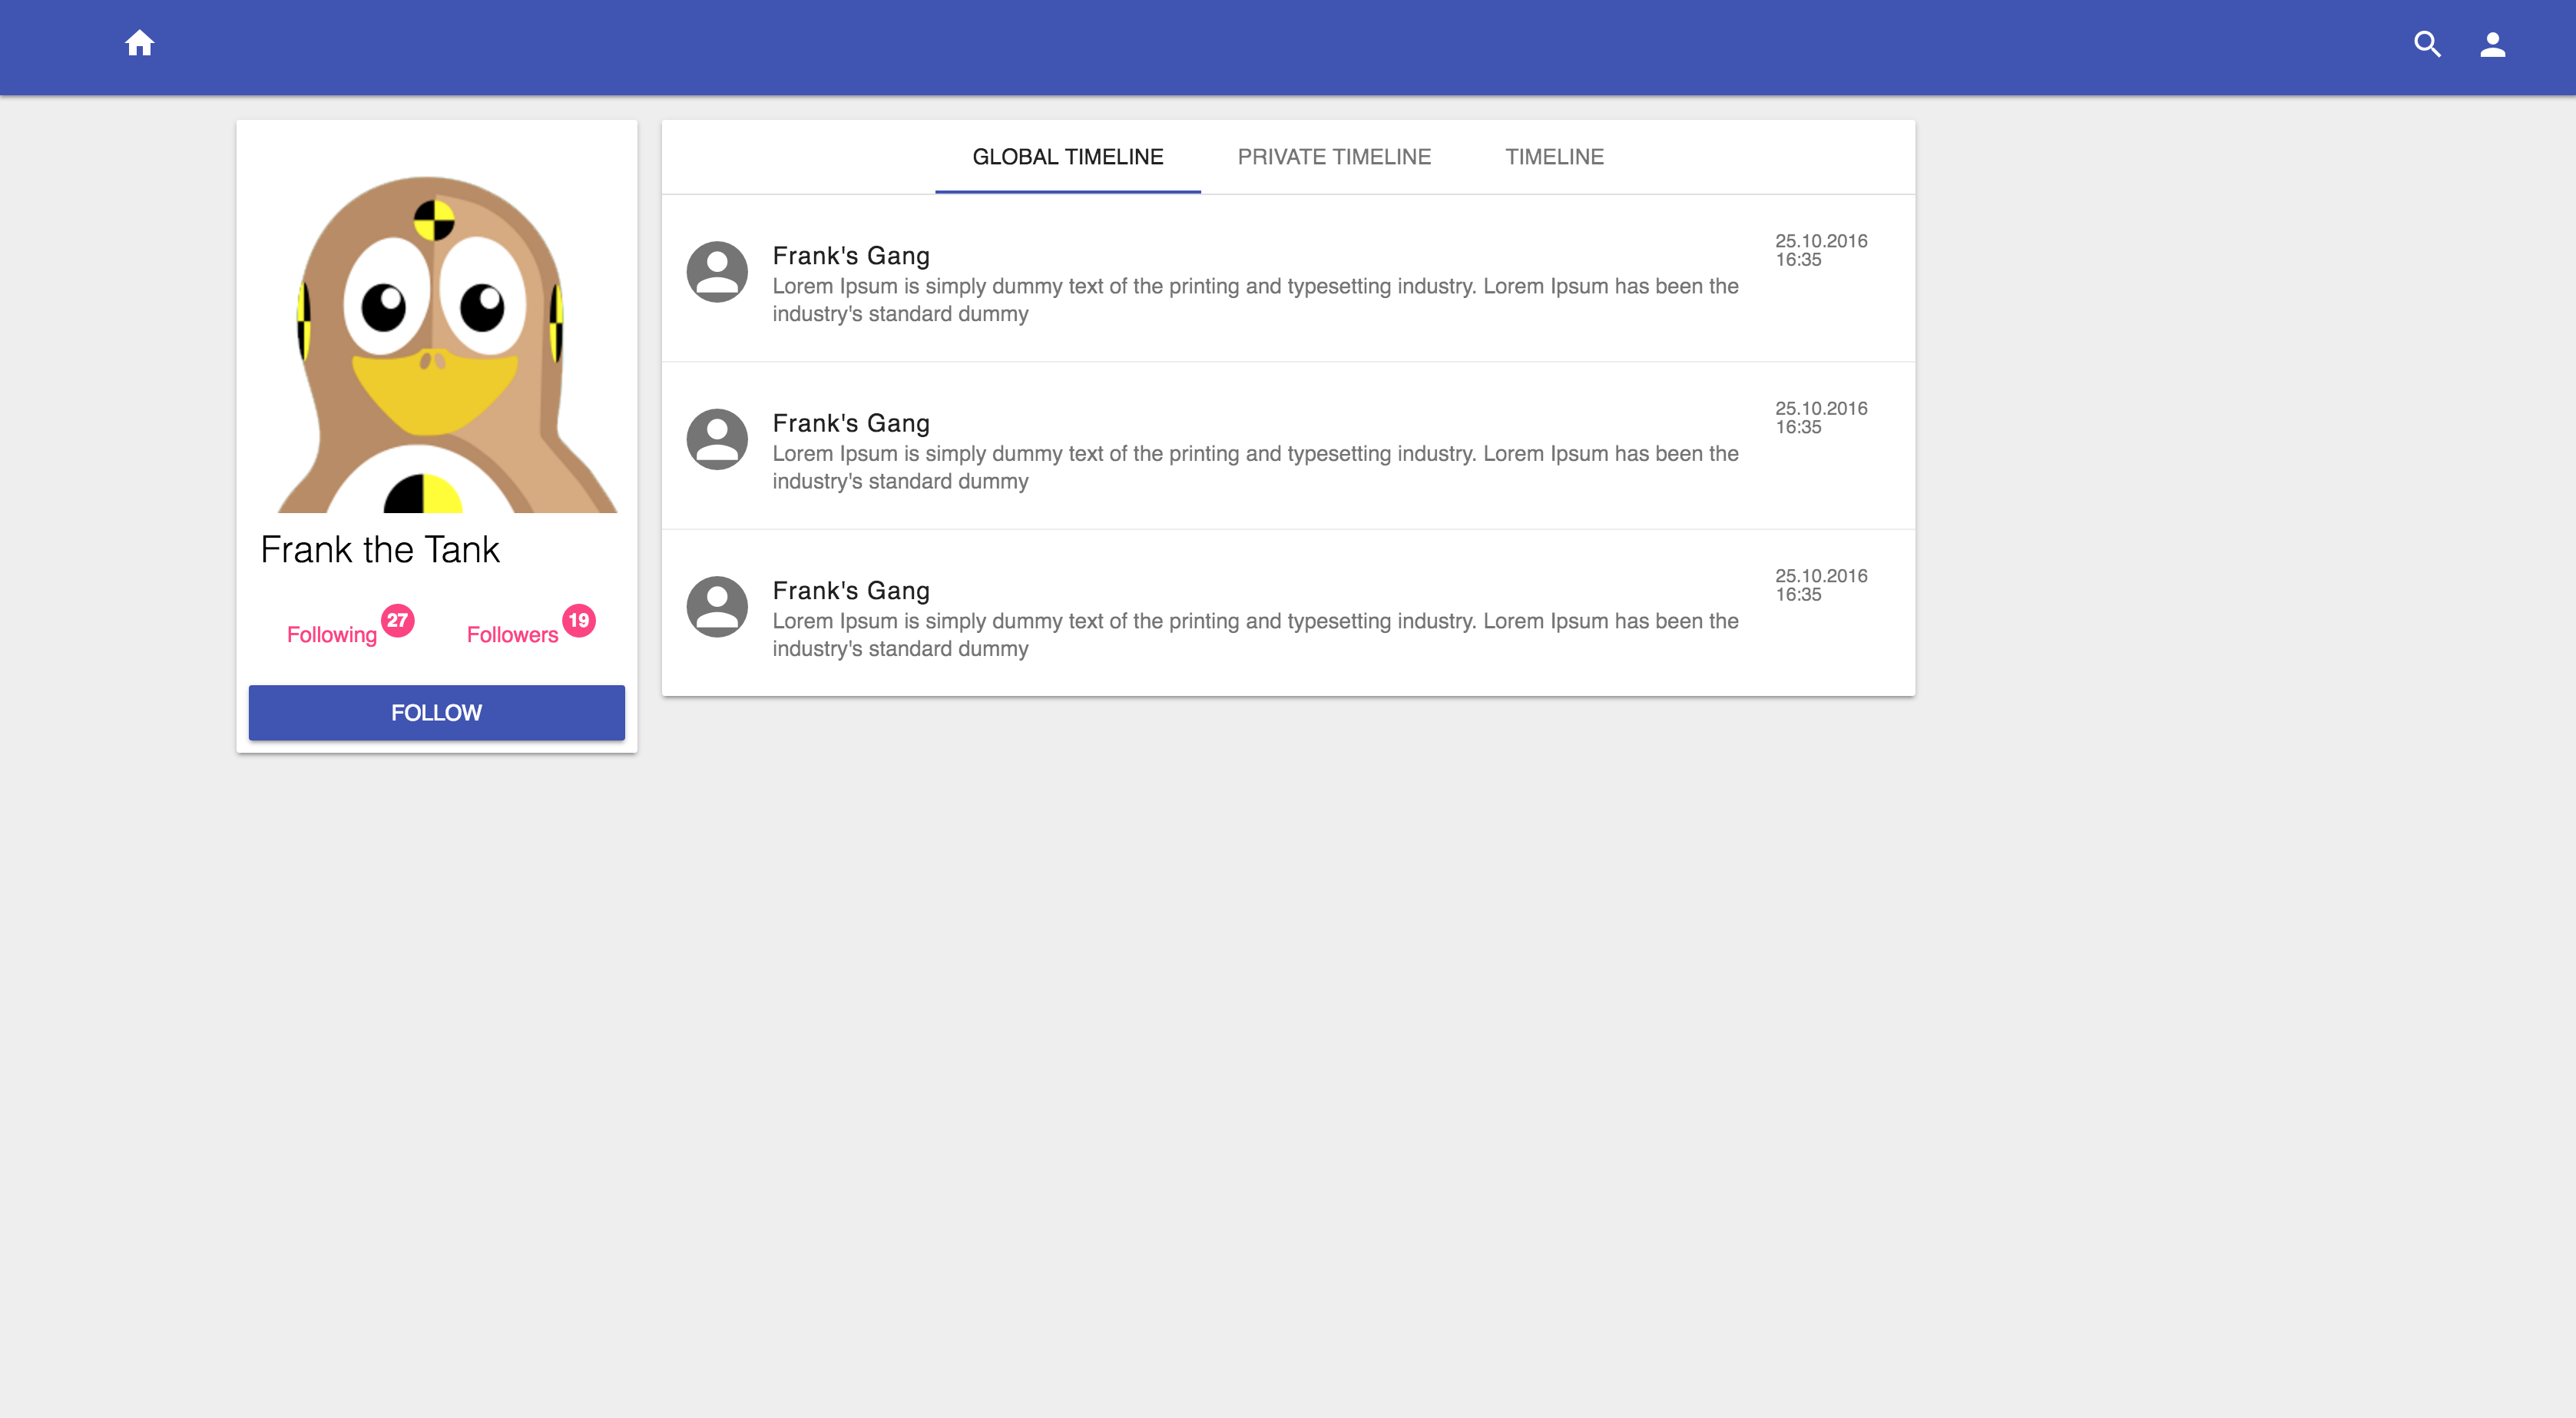
\includegraphics[width=\textwidth]{./images/1_user.png}
		Benutzeransicht\par\vspace{.6cm}
		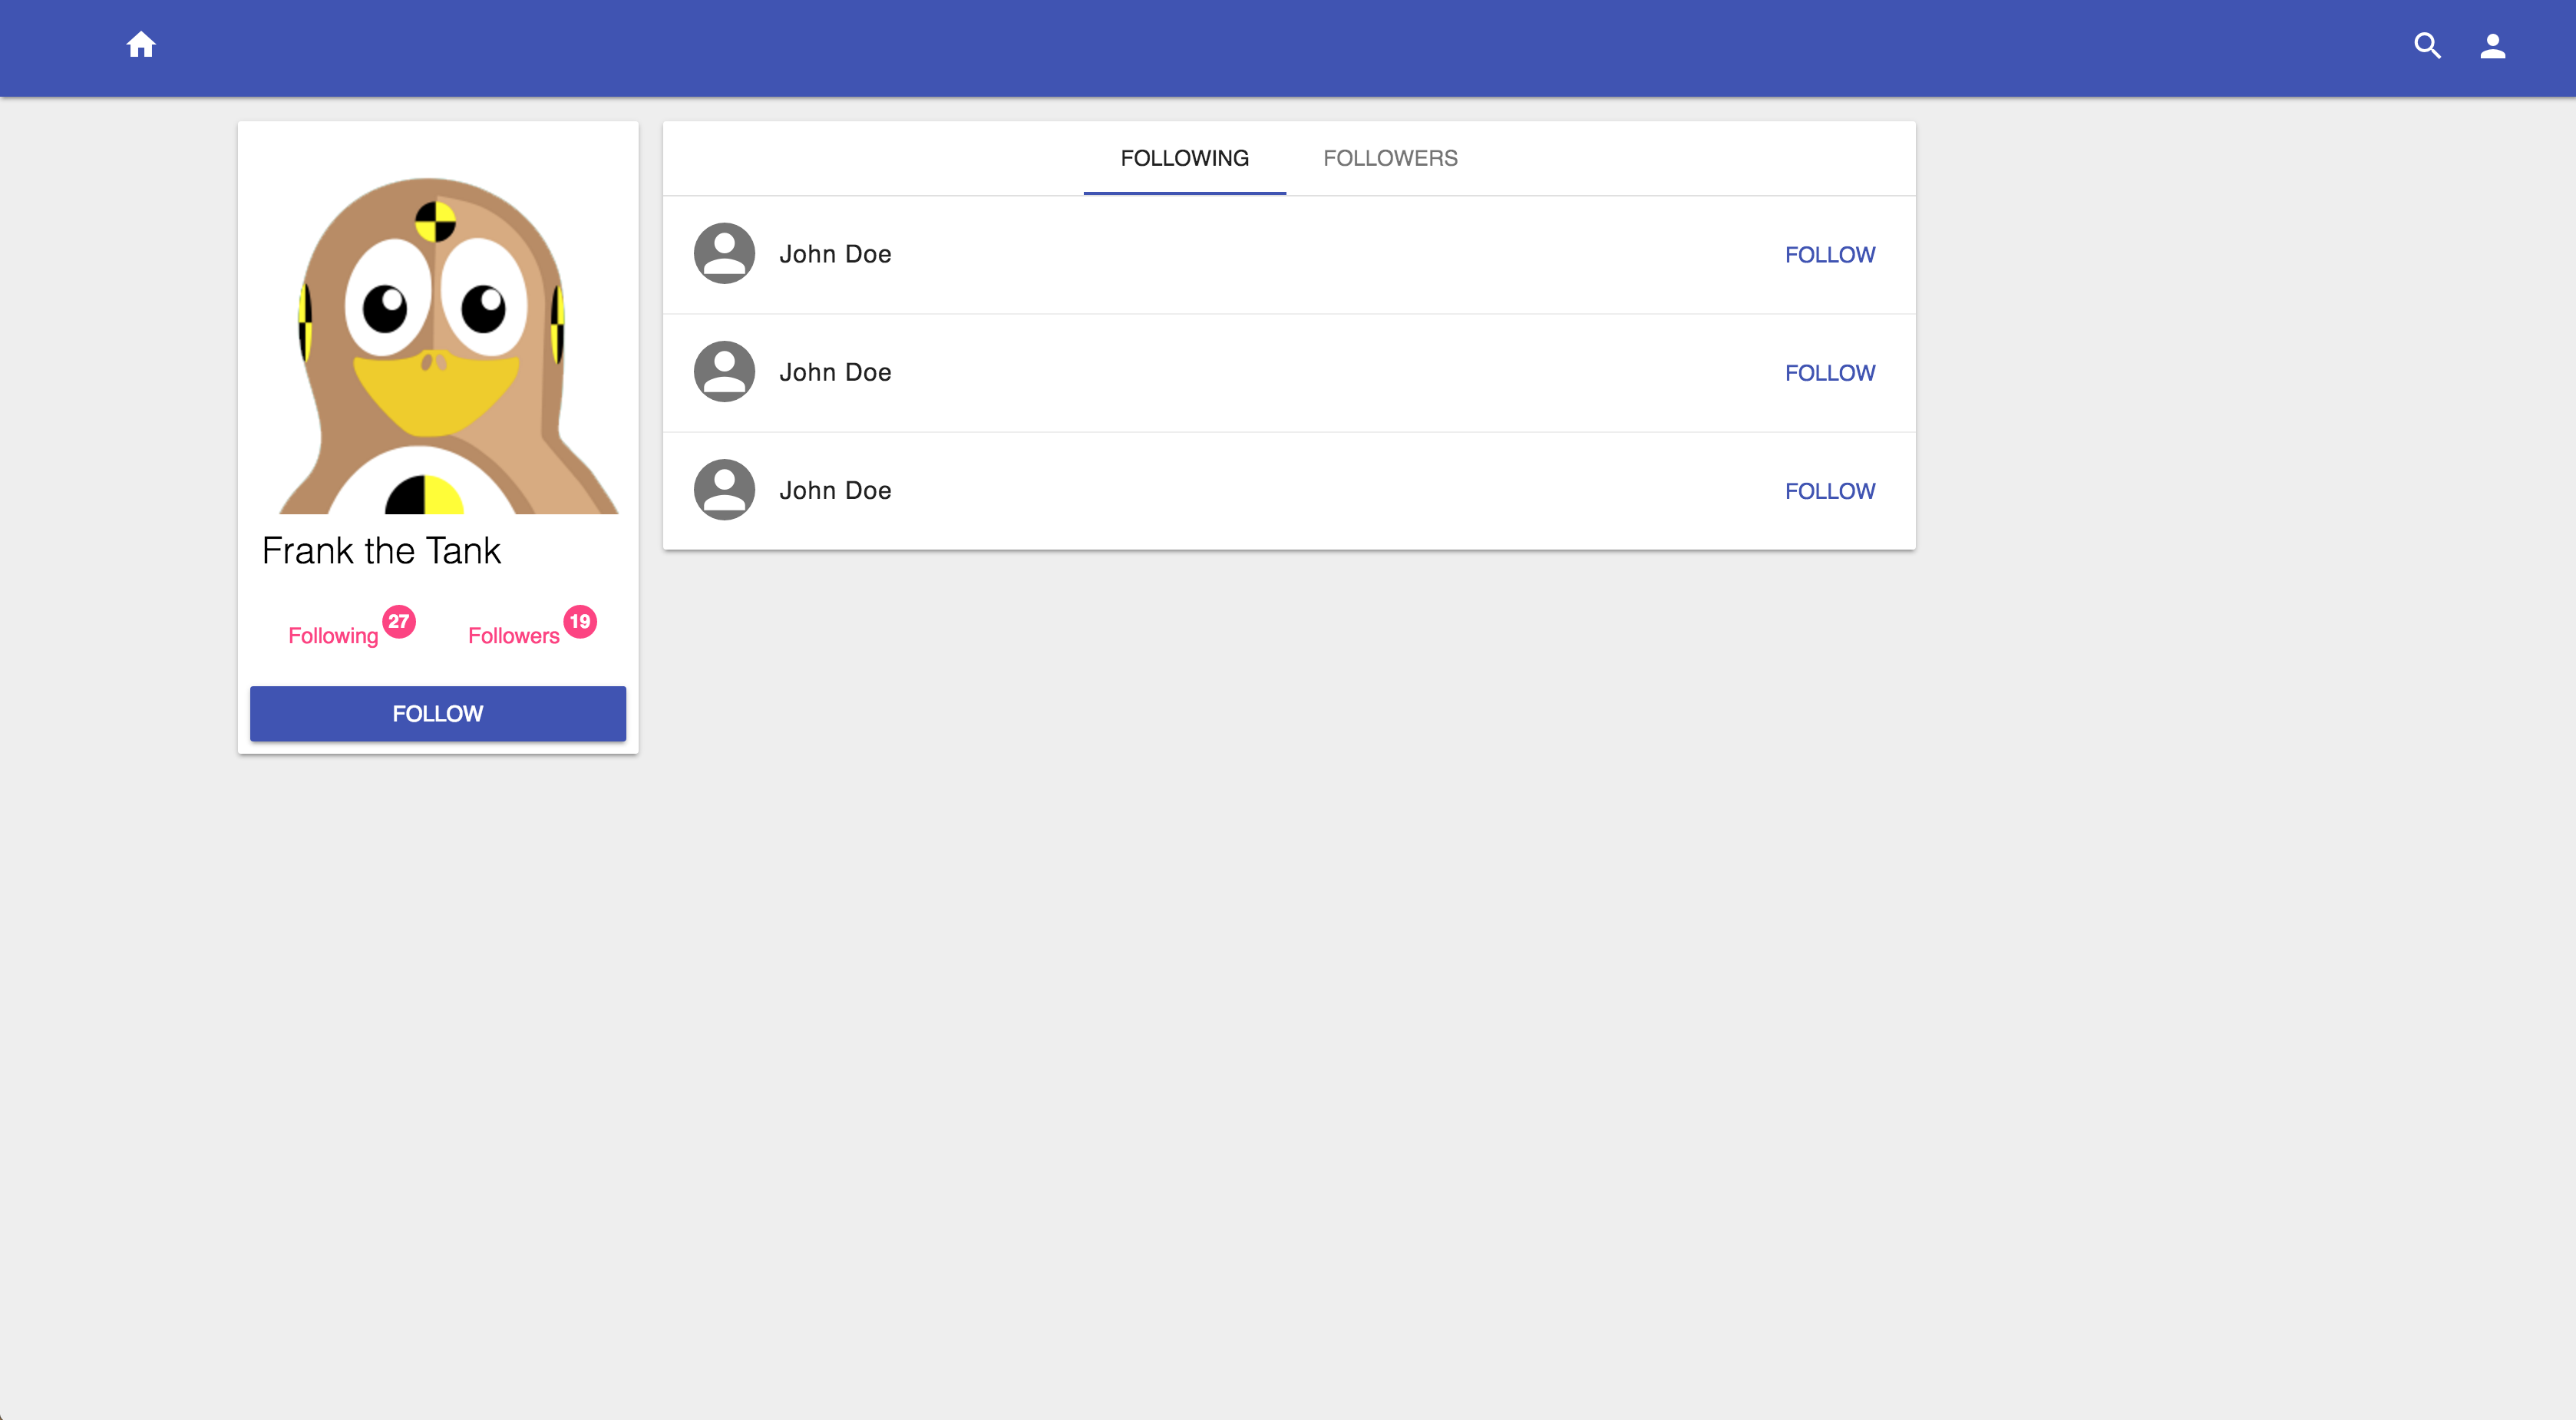
\includegraphics[width=\textwidth]{./images/1_user_followers.png}
		Followerliste des Benutzers

    \section{Datenmodell}
        \begin{lstlisting}[language=json]
//Set aller User
set user:all = {"essigt", "eirichg", "reesm", "blustt"}

//HashSets fuer die einzelnen Nutzer
hash user:*
    user:essigt = {id: "1", username: "essigt", firstname: "Tim", lastname: "Essig", password: "xyz", auth: "1aba56d8c5"}

//Sets um zu speichern, wer wem folgt
set user:*:follower
set user:*:following

//Keys um einen auth-token einem username zuzuordnen
key auth:*:username
    auth:1aba56d8c5:username = essigt

//Liste aller Posts
list post:all = {1,2,3,4}

//HashSets fuer die einzelnen Posts
hash post:*
    post:1 = {timestamp: 01-03-2016 13:37, message:"Meine tolle Nachricht", user:"essigt"}

list user:*:posts = {1} //Liste aller Posts eines Users
list timeline:* = {1,3} //Liste aller Posts der Follower des Users(incl. seiner eigenen)

//Globale Counter
key global:userid
key global:postid
        \end{lstlisting}


    % Aufgabe 2
    \chapter{Seitenbasierte Implementierung}
    \section{Redis Schnittstelle}
		Die Redis Schnittstelle ist in drei Repositories gegliedert, die für User, Post oder Authentifizierung verantwortlich sind, die alle Funktionalität aus ihrem Bereich bereitstellt. 
		\begin{itemize}
			\item UserRepository
			\item PostRepository
			\item AuthRepository
		\end{itemize}
		
		Die Konfiguration der Redis Datenbank(Host, Port und Passwort), wird in der RedisConfiguration-Klasse gehalten. Um die Konfiguration nicht ändern zu müssen, wenn man die Anwendung Lokal laufen hat(Host: Localhost) und in Docker(Host: redis). Hierzu wird auf eine Umgebungsvariable zurück gegriffen.
		\begin{lstlisting}[language=java]
String redisHost = System.getenv()
		.getOrDefault("REDIS_HOST", "localhost");
		\end{lstlisting}
		
    \section{Sessionverwaltung}
    Die Sessionverwaltung besteht aus vier Teilen:
    	\begin{itemize} 
    	\item LoginController
    	\item CookieInterceptor
    	\item SessionSecurity
    	\item Configuration
    \end{itemize}
\subsection{LoginController}
	Aktive Sessions werden in der Redis Datenbank gespeichert. Es wird ein Authentifizierungstoken mit dem entsprechenden (eindeutigen) Username verknüpft. Beim Login prüft der \textbf{LoginController}, ob Benutzername und Passwort korrekt sind, erstellt ggf. das Authentifizierungstoken und fügt es in die Datenbank ein. Des Weiteren wird das Token mit einem Timeout versehen, sodass es nach 10min automatisch aus der Datenbank gelöscht wird und die Session somit verfällt. Zuletzt wird das Token noch in einem Cookie abgelegt, damit für weitere Anfragen die Session bestehen bleibt.
	\begin{lstlisting}[language=java]
public class LoginController {
	
 @Autowired
 private AuthRepository repository;
 private static final Duration TIMEOUT = Duration.ofMinutes(10);

 public boolean login(User user, HttpServletResponse response) {
  if (repository.auth(user.getUsername(), user.getPassword())) {
   String auth = repository.addAuth(user.getUsername(), TIMEOUT.getSeconds(), TimeUnit.SECONDS);
   Cookie cookie = new Cookie("auth", auth);
   response.addCookie(cookie);
   SessionSecurity.set(user.getUsername(), auth);
   return true;
  }

  // Login not valid
  return false;
 }

 @RequestMapping(value = "/logout")
 public String logout() {
  if (isLoggedIn()) {
   String username = SessionSecurity.getName();
   repository.deleteAuth(username);
   SessionSecurity.clear();
  }

  return "redirect:/login";
 }

 public boolean isLoggedIn() {
  return repository.isAuthValid(SessionSecurity.getToken()).equals(SessionSecurity.getName());
 }
}
	\end{lstlisting}
	
	\subsection{CookieInterceptor}
	Sobald sich ein User eingeloggt hat, übernimmt der \textbf{CookieInterceptor}. Dieser wird bei Folgeanfragen ausgeführt und überprüft die Gültigkeit des Tokens. Ist es ungültig, erfolgt ein redirect zur Login-Seite.
	\begin{lstlisting}[language=java]
@Override
public boolean preHandle(HttpServletRequest req, HttpServletResponse res, Object handler) throws Exception {
Cookie[] cookies = req.getCookies();
if (!ObjectUtils.isEmpty(cookies))
 for (Cookie cookie : cookies)
  if (cookie.getName().equals("auth")) {
   String auth = cookie.getValue();
   if (auth != null && redis != null) {
    String username = redis.isAuthValid(auth);
    if (username != null) {
     SessionSecurity.set(username, auth);
     return true;
    }
   }
  }

  SessionSecurity.clear();
  res.sendRedirect("/login");
  return false;
}
	\end{lstlisting}
	
	\subsection{SessionSecurity}
	Die statische \textbf{SessionSecurity}-Klasse dient als lokaler Zwischenspeicher für den zuletzt verwendeten Token und Username. Im Kern hält die Klasse eine Threadabhängige Variable vom Typ SessionData:
	\begin{lstlisting}[language=java]
private static class SessionData {
String username;
String token;

 public SessionData(String un, String t) {
  username = un;
  token = t;
 }
}
	\end{lstlisting}
	
	\subsection{Configuration}
	Die \textbf{WebConfig}-Klasse dient zur Konfiguration des \textbf{CookieInterceptor}.
	\begin{lstlisting}[language=java]
@Configuration
public class WebConfig extends WebMvcConfigurerAdapter {


 @Override
 public void addInterceptors(InterceptorRegistry registry) {
  registry.addInterceptor(localeChangeInterceptor());
  registry.addInterceptor(cookieInterceptor()).excludePathPatterns("/login/**").excludePathPatterns("/registration/**").excludePathPatterns("/error/**");
 }

 @Bean
 public CookieInterceptor cookieInterceptor() {
  return new CookieInterceptor();
 }

 @Bean
 public LocaleChangeInterceptor localeChangeInterceptor() {
  return new LocaleChangeInterceptor();
 }
}
	\end{lstlisting}
	Die Konfiguration registriert den \textbf{CookieInterceptor}, sodass er bei jeder Anfrage von der Login- oder Register-Seite ausgeführt wird. Die beiden mit @Bean gekennzeichneten Factory-Methoden erlauben Spring die jeweiligen Objektinstanzen zu verwalten. Dadurch werden beide Objekte auch für Dependency Injection verfügbar.
	
    \section{MVC Implementierung}
    \subsection{Fronend}
	Um redundanten Code zu vermeiden, wurde die Templates in mehrere Fragment aufgeteilt. Thymeleaf bietet die Möglichkeit diese beim parsen einzubinden.
	
	Folgende Fragmente wurden erstellt:
	\begin{itemize} 
		\item Header
		\item Footer
		\item Profil/User
		\item Timeline
		\item Post
	\end{itemize}

	Auf jeder Seite, mit Ausnahme von \textbf{Login} und \textbf{Registrierung} werden die Komponente \textit{Header}, \textit{Footer} und \textit{Profil/User} eingebettet.
	
	In der Homepage und der Profilansicht wird zusätzlich die \textit{Timeline} eingebunden.\\
	
	\textbf{Beispiel: Profil/User - Fragment:}
	\begin{lstlisting}[language=html]
<div class="profile-card mdl-card mdl-shadow--2dp" th:fragment="card">
 <div id="profile-header" class="mdl-card__title">
  <h2 id="profile-name" class="mdl-card__title-text" th:text="${user.username}"></h2>
 </div>
		
 <div class="mdl-card__supporting-text">
  <a th:href="@{|/users/${user.username}/following|}" class="mdl-badge" th:attr="data-badge=${followingCnt}">Following</a>
  <a th:href="@{|/users/${user.username}/follower|}" class="mdl-badge" th:attr="data-badge=${followerCnt}">Follower</a>
 </div>
		
 <div class="mdl-card__actions" th:if="${!isSelf}">
  <a th:if="${!isFollowing}" th:href="@{|/follow/${user.username}|}" class="mdl-button mdl-button--raised mdl-button--colored mdl-js-button mdl-js-ripple-effect" style="width: 100%;">
   Follow
  </a>
  <a th:if="${isFollowing}" th:href="@{|/unfollow/${user.username}|}" class="warn mdl-button mdl-button--raised mdl-js-button mdl-js-ripple-effect" style="width: 100%;">
   Unfollow
  </a>
 </div>
</div>
	\end{lstlisting}
	\begin{lstlisting}[language=html]
<!--Profile-->
<div class="mdl-cell mdl-cell--2-col mdl-cell--4-col-phone">
 <div th:replace="components/profile :: card">...</div>
</div>
	\end{lstlisting}

    \subsection{Backend}
	Für jede View existiert ein Controller. Diese implementieren die RequestMappings für das jeweilige View. Die Controller füllen das Model und rendern das View.
	
	Zusätzlich wurden weitere Conroller erstellt, welche die Suche und das Folgen/Entfolgen implementieren.\\
	
	\textbf{Beispiel: LoginViewController:}
	\begin{lstlisting}[language=java]
@Controller
public class LoginViewController {

 @Autowired
 private LoginController loginController;

 @RequestMapping(value = "/login", method = RequestMethod.GET)
 public String showLoginView(Model model) {
  model.addAttribute("user", new User());

  return "login";
 }

 @RequestMapping(value = "/login", method = RequestMethod.POST)
 public String showLoginView(@ModelAttribute("user") User userForm, HttpServletResponse response, Model model) {

 if (userForm.getUsername() != null)
  if (userForm.getPassword() != null) {
   if (loginController.login(userForm, response)) {
    // Redirect user to home
    return "redirect:/";
   }
  }

  model.addAttribute("error", "Password or username is wrong.");
  return "login";
 }
}
	\end{lstlisting}

    % Aufgabe 3
    \chapter{Asynchrone Erweiterungen}
    \section{Push-Funktionalität}
    \subsection{Backend}
	Das Backend der Anwendung hat einen STOMP Endpoint an \textbf{/ws} registriert. Ebenso wie einen Broker \textbf{/topic}, über welchen die Nachrichten verteilt werden.
	
	Im MessageController werden die ankommen Nachrichten an \textbf{/post} verarbeitet, in diesem Fall werden neue Posts gespeichert und direkt an alle über \textit{WebSockets} verbundene Clients verteilt, die \textbf{/topic/posts} abboniert haben.
	
	\begin{lstlisting}[language=java]
@MessageMapping("/post")
@SendTo("/topic/posts")
public Post post(PostMessage postMessage) throws Exception {
 // Create and save post
 Post post = new Post(postMessage.getMessage(), postMessage.getUsername());
 postRepository.savePost(post);
 return post;
}
	\end{lstlisting}
	
	\subsection{Frontend}
	Im Client werden neue Post nicht mehr wie gehabt über \textit{POST} an das Backend gesendet, sondern als \textit{JSON} über eine \textit{WebSocket} Verbindung.
	
	Bei Aufrufen der Views, mit ausnahme von \textbf{login} und \textbf{registration} wird versucht eine \textit{WebSocket} verbindung an \textbf{/ws} aufzubauen und \textbf{/topic/posts} wird abboniert. 
	
	Jede Nachricht, die über das Socket ankommt ist ein neuer Post. 
	Befindet sich der User auf der \textbf{home} Seite, so wird der Post direkt in dessen Timeline eingefügt. Ist der User auf einer anderen View, so wird diesem eine Benachrichtigung angezeigt.
	
	Ist der Post von dem User, der es erstellt hat oder von einem User dem man folgt, so wird dieser auch in dessen \textbf{Privaten Timeline} eingebettet. 
	
	\begin{lstlisting}
function connect() {
 var hostname = window.location.hostname; 
 var port = window.location.port;
 var url = 'ws://' + hostname + ':' + port + '/ws';

 stompClient = Stomp.client(url);
 stompClient.debug = null; // Disable debug output
 stompClient.connect({}, function (frame) {
  console.log('Connected: ' + frame);
  stompClient.subscribe('/topic/posts', function (post) {
   postReceived(post)
  });
 });
}

function postReceived(post) {
 var obj = JSON.parse(post.body);

 if (path === '/') {
  if (obj.user === currentUser) { // Append to global AND private timeline
   appendPost(obj, true);
  } else {
   checkForFollower(obj)
  }
 } else if (path !== '/login' && path !== 'registration') {
  showNotification(obj);
 }
}

function checkForFollower(post) {
 var uri = '/isfollower?username=' + currentUser + '&follower=' + post.user;

 $.get(uri, function(response) {
 if (response.isFollower)
  appendPost(post, true);
 else
  appendPost(post);
 });
}
	\end{lstlisting}
 	
	\section{Redis Publish-Subscribe-Messaging}
	Das Publish-Subscribe Messaging sorgt für eine systemweite Benachrichtigung bei neuen Posts, sodass mehrere Serverinstanzen über einen neuen Post informiert werden können. 
	Zunächst muss der Server für das Publish-Subscribe Pattern konfiguriert werden:
	\begin{lstlisting}
@Configuration
public class PubSubConfiguration {

 public static final String postChannelName = "updates:post";

 @Autowired
 RedisConnectionFactory redisConnectionFactory;

 @Autowired
 RedisTemplate<String, Post> redisPostTemplate;

 @Bean
 MessageListenerAdapter messageListener() {
  return new MessageListenerAdapter(new MessageSubscriber());
 }

 @Bean
 RedisMessageListenerContainer redisContainer() {
  RedisMessageListenerContainer container
    = new RedisMessageListenerContainer();
  container.setConnectionFactory(redisConnectionFactory);
  container.addMessageListener(messageListener(), topic());
  return container;
 }

 @Bean
 MessagePublisher redisPublisher() {
  return new MessagePublisher(redisPostTemplate, topic());
 }

 @Bean
 ChannelTopic topic() {
  return new ChannelTopic(postChannelName);
 }
}
	\end{lstlisting}
	Die Konfiguration erstellt einen Publisher, der in dem Nachrichtenkanal \textit{updates:post} Nachrichten veröffentlicht. Die Implementierung des MessagePublishers veröffentlicht bei jedem Aufruf der \textit{publish(Post)} Funktion einen Post im Kanal \textit{updates:post}.
	
	\begin{lstlisting}
public class MessagePublisher {

 @Autowired
 private RedisTemplate<String, Post> redisPostTemplate;

 @Autowired
 private ChannelTopic topic;

 public MessagePublisher() {

 }

 public MessagePublisher(RedisTemplate<String, Post> template, ChannelTopic topic) {
  redisPostTemplate = template;
  this.topic = topic; 
 }

 public void publish(Post post){
  redisPostTemplate.convertAndSend(topic.getTopic(), post);
 }
}
	\end{lstlisting}
	Ein Subscriber kann nun den Kanal abonnieren, um die Benachrichtigungen des \textit{MessagePublisher} zu erhalten. Eine Beispielhafte Implementierung eines Subscribers wäre:
	\begin{lstlisting}
@Service
public class MessageSubscriber implements MessageListener {

 public static Stack<Post> recentPosts = new Stack<>();

 private final Logger logger = LoggerFactory.getLogger(this.getClass());

 public void onMessage(Message message, byte[] pattern) {
  try {
   ByteArrayInputStream bis = new ByteArrayInputStream(message.getBody());
   ObjectInputStream ois = new ObjectInputStream(bis);
   Post post = (Post) ois.readObject();
   recentPosts.push(post);
   logger.info("received post: " + post.toString());
   
   // Send to all clients
   this.sendPost(Post);
  } catch (Exception e) {
   logger.error("can't convert message to Post, message: " + message.toString());
  }
 }
}
	\end{lstlisting}
	Dieser Subscriber deserialisiert die Nachricht und konvertiert sie in ein Objekt vom Typ \textit{Post}. Anschließend legt er den Post auf einen Stack, welcher die neuesten Nachrichten beinhaltet. 
	
	Anschließen werden die neuen Posts an alle verbunden Clients gesendet.
	\begin{lstlisting}
private void sendPost(Post post) throws Exception {
 this.template.convertAndSend("/topic/posts", post);
}
	\end{lstlisting}
\end{document}
